\documentclass[../main.tex]{subfiles}
\begin{document}

\section{Calibrations and exogenous variables}
\label{sec:calibrations}
The model is calibrated for the Danish economy, and the world interest rate is generated within the same model setup for the non-Euro Area (EA) G7 countries (Canada, Japan, UK and USA).\footnote{We chose this group of countries mostly because of data availability and simplicity, as the world interest rate is already generated in \textcite{bielecki2020demographics}. However, these four similarly developed countries seem a fair representation of cross-border economic interactions from a Danish economy perspective in determining the world interest rate.} We simulate the model using Dynare in MatLab, a popular software tool used by academics for handling Dynamic Stochastic General Equilibrium (DSGE) and life-cycle models.\footnote{For more information, see \textcite{Adjemianetal2011}.  We provide the calibrated main Dynare code in Appendix \ref{sec:Dynare_code_appendix}.} Below, we describe data, both demographic and life-cycle microdata, used in our simulations. Furthermore, we describe structural parameters and exogenous forces used for calibrating the model.

\subsection{Life-cycle characteristics}
\label{sec:life-cycle_characteristics}
To obtain knowledge on life-cycle behaviour and characteristics, we have gained access to Danish registry data and The Danish Consumption Survey through The Economic Council of the Labour Movement in Denmark.

Access to The Danish Consumption Survey allows us to incorporate data on the average consumption for each cohort. The Danish Consumption Survey is a survey with a reduced sample size compared to registry data, but it enables the possibility of limiting consumption to the amount spent on food and utilities (water, electricity and heating). We use aggregated consumption from 2014-2018 to gain a larger sample and overcome potential outliers. Values are deflated by the 2018 price level. All data is extracted at household levels and determined by the head of the household, defined as the one with the highest income. To account for different household sizes, we use an equivalence scale of 0.6 in line with recent literature on methods of accounting for these differences while working with household-level data  (\cite{fernandez2007consumption}). We use Danish registry data on hourly wages, labour income, and net wealth. To match the age profiles in the model, data on household heads for each cohort has been collected. Net wealth is excluding occupational or public pension benefits and is denoted "assets" in line with the terminology used previously in the model. Values have been deflated by the 2019 price level.

The empirical measure of labour productivity $z_j$ is hourly labour income, including wage and self-employment. The data profile is smoothed with a Hodrick-Prescott filter explaining the minor deviations between data and the exogenous productivity input illustrated in Figure \ref{fig:Life_cycle}\textcolor{blue}{A}.\footnote{Like \textcite{bielecki2020demographics}, we keep the smoothing parameter consistently at 100 throughout the paper.} Productivity tends to increase until the household head is reaching the age of 50 before it starts to decrease marginally. When agents reach their 60s, we see a tendency of increased productivity. It is important to emphasize that if productivity is measured as the hourly wage, it can obviously be affected by benefits given to workers deciding to extend their period of working. Thus, this increase in productivity is more likely to indicate a need for extended labour than an increase in actual productivity for each individual.

Even though we do not specifically target the life-cycle characteristics, in particular consumption and net wealth, Figure \ref{fig:Life_cycle}\textcolor{blue}{B} and \ref{fig:Life_cycle}\textcolor{blue}{C} illustrate how well our model captures the development over time. The household-weighted consumption increases slightly on average as people age. Assets are close to zero when agents are 25 and increase heavily until retirement age. Hereafter, assets are converging towards zero. While data does not indicate a convergence towards zero for assets, there is a clear tendency of a decline in assets for retirees, and our model predictions for 25-65 years old seem to match actual data remarkably well.

\begin{figure}[H]
    \centering
    \caption{Life cycle characteristics}
    \label{fig:Life_cycle}
    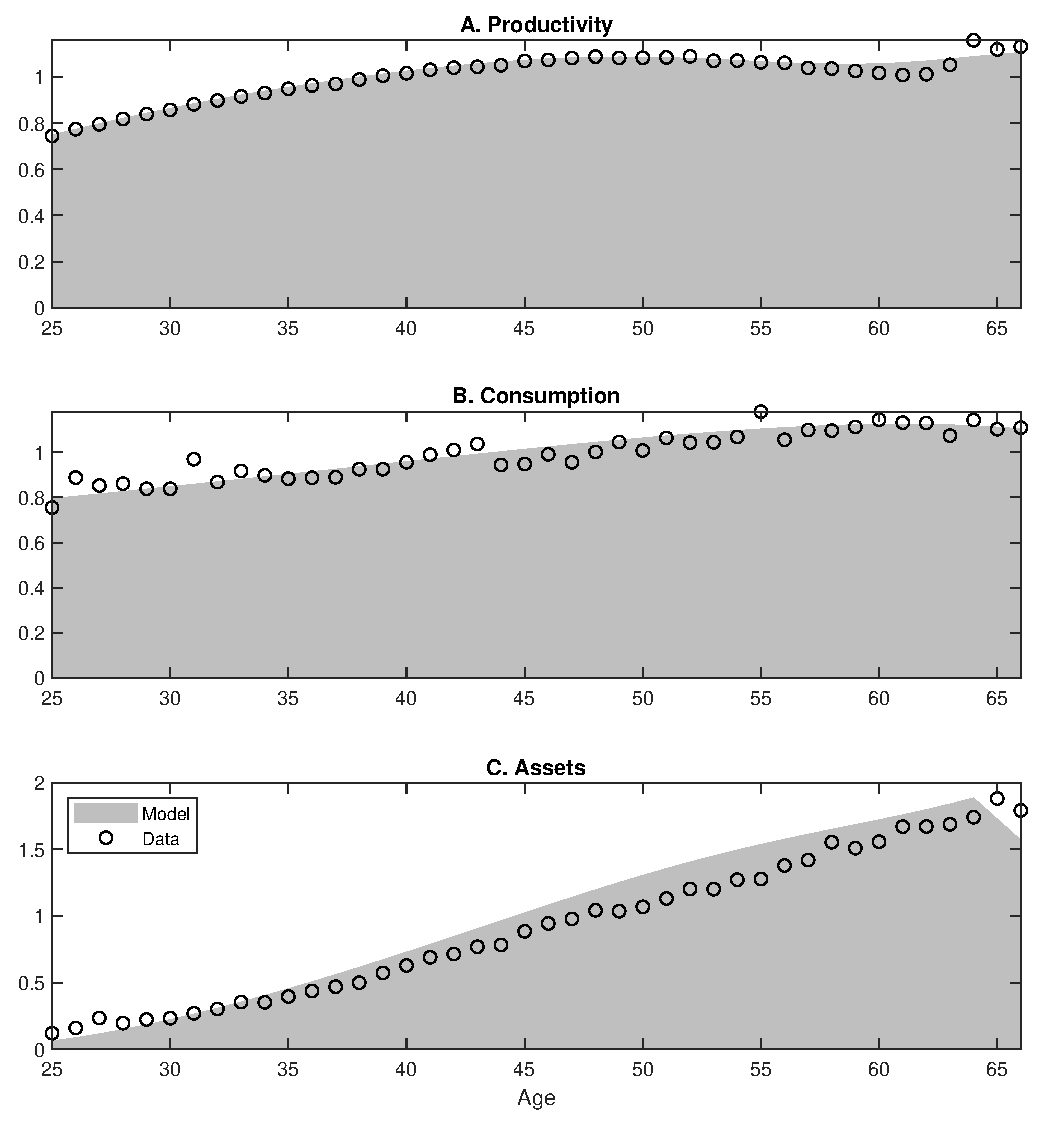
\includegraphics[scale=0.7]{Figures/Figure_2.eps}\\
       \begin{fignote}
           \textit{Note:} Life-cycle profiles from The Danish Consumption Survey and Danish registry data obtained with the help of The Economic Council of The Labour Movement. Values have been normalized by the mean.
       \end{fignote}    
\end{figure}

\subsection{Demographics}
Demographic shocks to the model are based on projections and actual mortality rates by \cite{WorldPop12:online}, World Population Prospects that cover the period from 1950-2100. Since mortality data from the UN is only available on 5 year age intervals, we follow \textcite{bielecki2020demographics} and use cubic splines to interpolate to annual and 1 year age frequency. Subsequently, the resulting mortality rates and cohort sizes of 20 year olds are then smoothed by the Hodrick-Prescott filter to isolate the structural demographic development. See table \ref{tab:cohort_construction} below for illustration:
\begin{table}[H]
\centering
\caption{Cohort construction}
\label{tab:cohort_construction}
\begin{threeparttable}
\resizebox{\textwidth}{!}{\begin{tabular}{|c|c|c|c|c|}
\hline
\textbf{} & \textbf{20}   & \textbf{21}                                      & $\dots$  & \textbf{99}                                         \\ \hline
1900      & $n_{1,t}$     & $n_{2,t}$                                        & $\dots$  & $n_{80,t}$                                          \\ \hline
1901      & $\frac{N_{1,t+1}}{N_{1,t}}=n_{1,t+1}$   & $n_{2,t+1}=n_{1,t}\cdot(1-\omega_{1,t})$         & $\ddots$ & $n_{80,t+1}$                                        \\ \hline
$\vdots$  & $\vdots$      & $\ddots$                                         & $\ddots$ & $\vdots$                                            \\ \hline
2000      & $\frac{N_{1,t+100}}{N_{1,t+99}}=n_{1,t+100}$ & $n_{2,t+100}=n_{1,t+99}\cdot(1-\omega_{1,t+99})$ & $\ddots$  & $n_{80,t+100}=n_{79,t+99}\cdot(1-\omega_{79,t+99})$ \\ \hline
$\vdots$  & $\vdots$      & $\ddots$                                         & $\ddots$ & $\vdots$                                             \\ \hline
\end{tabular}}
        \end{threeparttable}
        \end{table}
We follow the authors and start our simulations in 1900 to avoid contamination of initial conditions. As we do not have data from 1900-1950, we construct it artificially.\footnote{Given the overall good data availability in Denmark, we could potentially have used a different source. But to avoid splicing data sets, we instead constructed it artificially with UN data we already use.} This is done by backcasting the size of 20-year cohort size holding mortality rates from 1970 constant to arrive at a population structure as close to reality as possible. Naturally, due to migration, it is impossible to match the exact demographic development, but in choosing 2010 as our base year, we avoid a recent major inflow of migration in 2015.\footnote{See \textcite{MFA_refugee_crisis_2015}} As a result, the constructed data does not seem far off reality (see Figure \ref{fig:demographics}). 
    \begin{figure}[H]
        \centering
        \caption{Model population}
        \label{fig:demographics}
        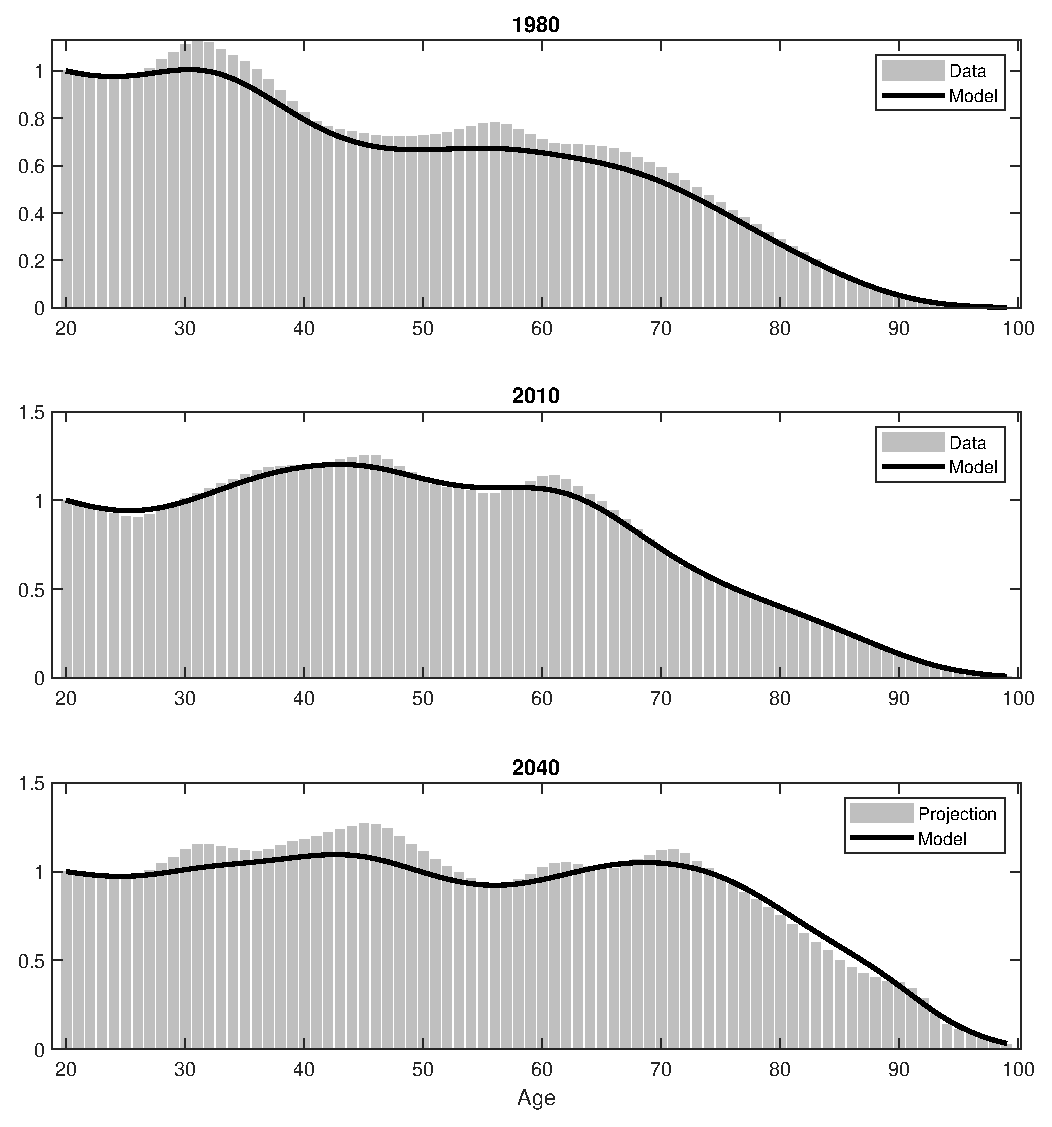
\includegraphics[scale=0.7]{Figures/Figure_3.eps}
        \\\begin{fignote}
            \footnotesize \textit{Note}: Calculations using Python code kindly shared by Marcin Bielecki on data from UN. Cohort sizes have been normalized by the size of the 20-year-old cohort. 
        \end{fignote}
    \end{figure}

\subsection{Exogenous forces}
Besides demographics, we feed into our model an exogenous measure for TFP, which has been discussed as an important driver for the NRI in recent literature (\textcite{rachel2015secular}). We define it as the world technology frontier $x_t$ in line with \textcite{bielecki2020demographics}. The time series is constructed using a GDP-weighted TFP index for 1960-2020 for non-EA G7 countries and then spliced with projections for the Euro Area (EA) 2016-2070 from the Aging Working Group. Thus, the growth rate of potential TFP is the same for Denmark as it is for non-EA G7 countries.\footnote{We cross-check this with data for TFP growth from Statistikbanken, table NP25, spanning the years 1967-2019. The trend is mostly the same.}

Data for public debt is extracted from the IMF WEO database. Like \textcite{bielecki2020demographics}, we choose net debt and not gross debt since gross debt, amongst other factors, include debt that a government owes to itself. As data for Denmark is only available between 1995-2024, while EA data exists from 1980-2024, we assume that the development of net public debt in Denmark between 1980 and 1995 follows the EA. Years preceding 1980 are kept at the 1980 EA level, and years following 2024 are kept at Danish 2024 levels. The Hodrick-Prescott filter is applied to smooth fluctuations due to business cycles. Government expenditures are fixed to 25 percent of GDP given a relatively little time variation in recent times (2000-2020).\footnote{Source: Table NAN1, Statistikbanken} The replacement rate $\varrho_t$ is fixed to 42 percent which corresponds the to value observed from 2015-2020.\footnote{Source: \textcite{pension_system_replacement_rate}} For non-EA G7 countries the retirement age is set to 63 to reflect retirement policy in the respective countries (\textcite{bielecki2020demographics}). 

Figure \ref{fig:TFP_DepRatio_NetPublicDebt}\textcolor{blue}{B} shows the past realizations and projections for TFP, the dependency ratio and net public debt that exogenously drive the model. The demographic transition unsurprisingly leads to a higher dependency ratio, defined as the ratio between retirees and workers, reflecting lower mortality and fertility. Starting from around 28 percent in 1980, a fixed retirement age of 65 in Denmark leads to a dependency ratio above 50 percent in 2040 and beyond. 

The growth rate of TFP substantially declined from the late 1980s until the global financial crisis around 2008-2009 but is expected to rebound heading into the near future. However, it is not expected to reach the growth rates of the late 1980s to early 1990s until after 2040. Furthermore, Danish debt levels are substantially lower than those of non-EA G7 countries. 

\begin{figure}[H]
    \centering
    \caption{Key exogenous driving forces}
    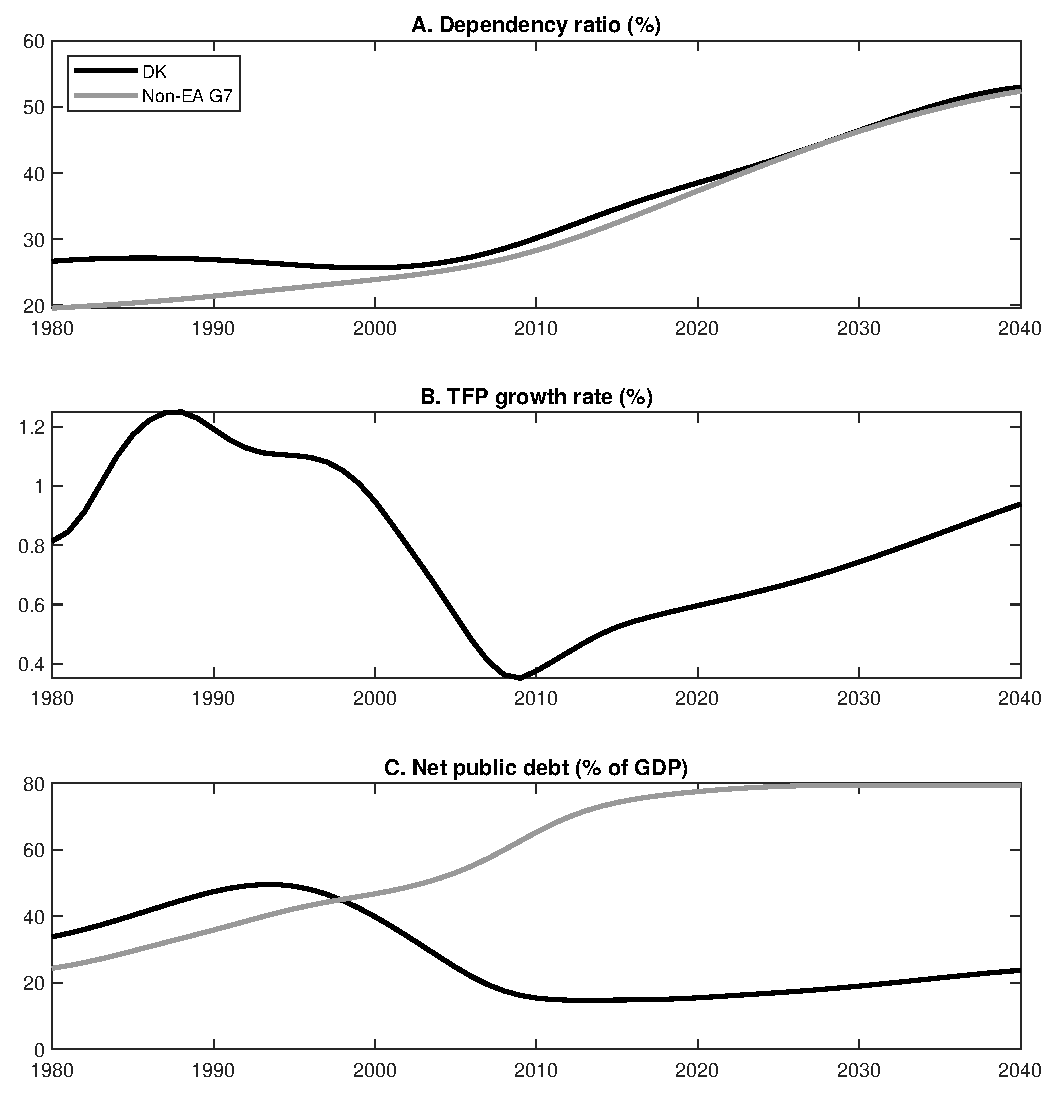
\includegraphics[scale=0.8]{Figures/Figure_5.eps}
    \label{fig:TFP_DepRatio_NetPublicDebt}\\
       \begin{fignote}
           \textit{Note:} Dependency ratio is defined as the ratio between retirees and workers. Recall that the retirement age in Denmark is higher (65) than in the non-EA G7 countries (63).
       \end{fignote}
\end{figure}

\subsection{Structural parameters}
The structural parameters used to calibrate the model to match available data are reported in table \ref{tab:Calibrated_parameters}. The discount factor $\beta$ is calibrated to $1.0082$ to target the average real interest rate of 1 percent in Denmark from 2000-2007, defined as Nationalbanken's nominal interest rate \textit{diskonto} minus inflation (consumer price index).\footnote{Source: Tables PRIS8 and DNRENTA, Statistikbanken} Around this time, the economy can be considered to be somewhat close to equilibrium with a stable inflation of around 2 percent. An important point here is that the fall of interest rates after the the global financial crisis in 2008-2009 should be attributed to cyclical rather than structural reasons. 

For the closed model that generates the world interest rate, $\beta^*$ is calibrated to $1.0093$ to match real interest rates of $0.8$ percent observed in the non-EA G7 countries in 1999-2008.\footnote{This is in line with \textcite{bielecki2020demographics}. However, when targeting $\beta$, we choose the period from 2000-2007 to make sure we do not capture the cyclical impact of the low interest rates during the global financial crisis and the early dot-com bubble.}

Like \textcite{bielecki2020demographics} and standard literature, capital depreciation rate $\delta$ is set to 10 percent annually and the product markup $\mu$ is set to 1.25.  Capital's share of output $\alpha$ is set to 0.25, which ensures a labour income share of 60 percent, in line with data, see \textcite{birch2010introducing}:\footnote{See derivations in Appendix \ref{sec:appendix_labour_cap_income_share}.}
\begin{align*}
    \frac{w_th_t}{y_t}=\frac{1-\alpha}{\mu}
\end{align*}
The risk premium $\xi$ is calibrated to $0.02$ by targeting Denmark's average net foreign assets of $-8$ percent of GDP from 2000-2007. 

\begin{table}[H]
\centering
\caption{Calibrated parameters}
\label{tab:Calibrated_parameters}
\begin{threeparttable}
\begin{tabular}{lllll}
\hline
\textbf{Parameter} & \textbf{Value} & \textbf{Description} \\ \hline
$\beta$          & $1.0082$          & Discount factor in DK \\ \hline
$\beta^*$          & $1.0093$          & Discount factor in non-EA G7 \\ \hline
$\delta; \delta^*$          & $0.1$          & Capital depreciation rate \\ \hline
$\alpha; \alpha^*$          & $0.25$          & Capital share in output \\ \hline
$\mu; \mu^*$          & $1.25$          & Product markup \\ \hline
$\xi$          & $0.02$          & Risk premium \\ \hline
\end{tabular}
    \end{threeparttable}
\end{table}

\end{document}
